\documentclass[12pt]{article}
\usepackage{url,graphicx,tabularx,array,geometry,enumitem,amsmath}
\setlength{\parskip}{1ex} %--skip lines between paragraphs
\setlength{\parindent}{0pt} %--don't indent paragraphs

%-- Commands for header
\renewcommand{\title}[1]{\textbf{#1}\\}
\renewcommand{\line}{\begin{tabularx}{\textwidth}{X>{\raggedleft}X}\hline\\\end{tabularx}\\[-0.5cm]}
\newcommand{\leftright}[2]{\begin{tabularx}{\textwidth}{X>{\raggedleft}X}#1%
& #2\\\end{tabularx}\\[-0.5cm]}
\def\ci{\perp\!\!\!\perp}


%\linespread{2} %-- Uncomment for Double Space
\begin{document}

\title{Digital Signal Processing - Assignment 8}
\line
\leftright{\today}{Stephanie Lund (2555914)\\Stalin Varanasi (2556235)} %-- left and right positions in the header

\section*{Exercise 1}

\subsection*{1.1}
We can use the error function:
\begin{align*}
e(n) = s(n) - \hat{s}(n) = s(n) - h(n) \ast x(n)
\end{align*}

converted to the frequency domain to find $J(\omega)$. Using the properties of additivity, and that convolution in the time domain is multiplication in the frequency domain, this is:
\begin{align*}
J(\omega) = S(\omega) - H(\omega)X(\omega)
\end{align*}

\subsection*{1.2}
\begin{align*}
E[J(\omega)^2] &= E[(S(\omega) - H(\omega)X(\omega))^2] \\\\
&= E[(S(\omega))^2 - 2S(\omega)H(\omega)X(\omega) + (H(\omega)X(\omega))^2] \\\\
\frac{\partial J}{\partial H(\omega)} &= E[-2S(\omega)X(\omega) + 2H(\omega)X(\omega)] = 0
\end{align*}

TODO: finish this

\subsection*{1.3}
From $X(\omega) = S(\omega) + N(\omega)$, we have:
\begin{align*}
H(\omega) &= \frac{\Phi_{sx}(\omega)}{\Phi_{xx}(\omega)} \\ \\
&=
\frac{E[X(\omega)S(\omega)] - E[X(\omega)]E[S(\omega)]}{E[X(\omega)^2] - E[X(\omega)]^2}\\ \\
&=
\frac{E[(S(\omega) + N(\omega))S(\omega)] -  E[(S(\omega) + N(\omega))]E[S(\omega)]}
{E[(S(\omega) + N(\omega))^2] - E[(S(\omega) + N(\omega))]^2} \\ \\
&=
\frac{E[(S(\omega)^2] + E[N(\omega)S(\omega)] -  (E(S(\omega)]^2 + E[N(\omega)S(\omega)])}
{E[S(\omega)^2] + 2E[S(\omega)]E[N(\omega)] + E[N(\omega)^2] - (E[S(\omega)]^2 + 2E[S(\omega)]E[N(\omega)] + E[N(\omega)]^2)} \\ \\
&=
\frac{\Phi_{ss}(\omega)}
{\Phi_{ss}(\omega) + \Phi_{nn}(\omega)}
\end{align*}

\subsection*{1.4}

We can multiply the frequency response $H(\omega)$ by the Fourier transform of the input $X(\omega)$ to get the result in the frequency domain, then take the inverse Fourier transform to find the denoised signal in the time domain $\hat{s}(n)$.

\subsection*{1.5}
Using the equation from question $1.3$, this is:

\begin{align*}
H(\omega) &= \frac{\Phi_{ss}(\omega)}
{\Phi_{ss}(\omega) + \Phi_{nn}(\omega)} \\ \\
&= \frac{\Phi_{ss}(\omega) / \Phi_{nn}(\omega)}
{\Phi_{ss}(\omega) / \Phi_{nn}(\omega) + \Phi_{nn}(\omega) / \Phi_{nn}(\omega)} \\ \\
&= \frac{SNR_k}{SNR_k + 1}
\end{align*}

\subsection*{1.6}

For $SNR_k$ in the range $[0, 30]$, using the above equation we get the frequency responses:\\
$[ 0    ,  0.5       ,  0.66666667,  0.75      ,  0.8       ,
        0.83333333,  0.85714286,  0.875     ,  0.88888889,  0.9       ,
        0.90909091,\\0.91666667,  0.92307692,0.92857143,  0.93333333,
        0.9375    ,  0.94117647,  0.94444444,  0.94736842,\\  0.95      ,
        0.95238095,  0.95454545,  0.95652174,  0.95833333,  0.96      ,
        0.96153846,  0.96296296,  0.96428571,\\0.96551724,  0.96666667,
        0.96774194]$ \\ \\
        
  If we take $20*log(H(\omega) + \epsilon)$ (where $\epsilon$ is a small number to prevent taking the log of 0) and plot it against $SNR_k$, we get the following graph:

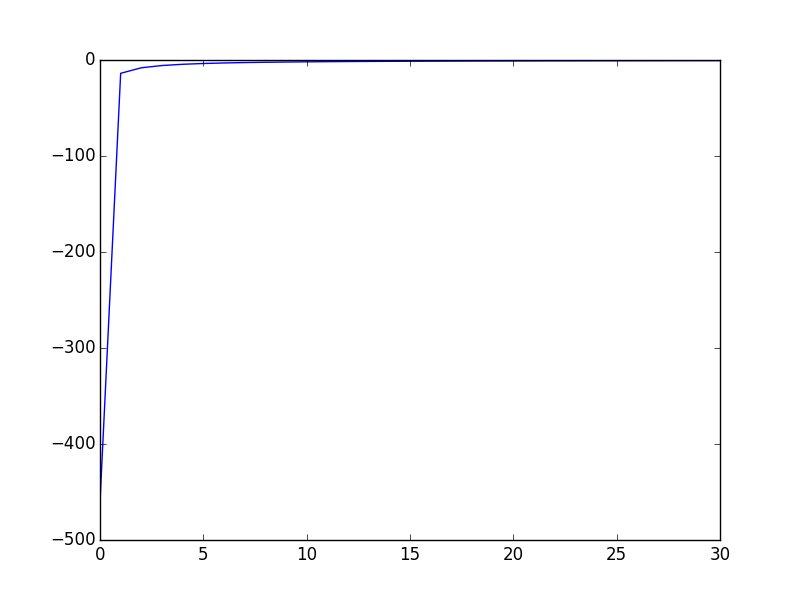
\includegraphics[scale=0.7]{hw8.png}
\end{document}